\section{Sejarah Python}
Bahasa pemrograman Python adalah bahasa yang dibuat oleh seorang keturunan Belanda yaitu Guido van Rossum. Sampai saat ini Python masih dikembangkan oleh \textit{Python Software Foundation}. Awalnya, pembuatan bahasa pemrograman ini adalah untuk membuat skrip bahasa tingkat tinggi pada sebuah sistem operasi yang terdistribusi Amoeba. Python telah digunakan oleh beberapa pengembang dan bahkan digunakan oleh beberapa perusahaan untuk pembuatan perangkat lunak komersial. Pemrograman bahasa python ini adalah pemrogram gratis atau \textit{freeware}, sehingga dapat dikembangkan, dan tidak ada batasan dalam penyalinannya dan mendistribusikan. 

Python dikembangkan oleh Guido van Rossum pada akhir tahun delapan puluhan dan awal tahun sembilan puluhan di National Research Institute for Mathematics and Computer Science di Belanda. Python berasal dari banyak bahasa lain, termasuk ABC, Modula-3, C, C ++, Algol-68, SmallTalk, dan shell Unix dan bahasa script lainnya.
Fitur overview terbaik adalah IT mendukung metode pemrograman fungsional dan terstruktur serta OOP. Hal ini dapat digunakan sebagai bahasa scripting atau dapat dikompilasi untuk byte-kode untuk membangun aplikasi besar. Ini memberikan tingkat yang sangat tinggi pada tipe data dinamis dan mendukung memeriksa jenis dinamis. IT mendukung pengumpulan sampah otomatis. Hal ini dapat dengan mudah diintegrasikan dengan C, C ++, COM, ActiveX, CORBA, dan Java. Hal tersebut menjadi terpopuler karena kemudahan bagi programmer yang menjadikan python pemograman terbaik pada tahun 2016.

Saat ini pengembangan Python terus dilakukan oleh sekumpulan pemrogram yang dikoordinir Guido dan Python Software Foundation. Python Software Foundation adalah sebuah organisasi non-profit yang dibentuk sebagai pemegang hak cipta intelektual Python sejak versi 2.1 dan dengan demikian mencegah Python dimiliki oleh perusahaan komersial. Saat ini distribusi Python sudah mencapai versi 2.7.14 dan versi 3.6.3. 

\section{Muhammad Fahmi}

\subsection{Sejarah Pyton}
Guido Van Rossum adalah orang yang menciptakan python di Scitching Mathematisch Centrum (CWI) Belanda pada wal tahun 1990-an. 
Pada nama python sendiri berasal dari nama ular yang kita tau. Guido Van Rossum seorang yang menggemarkan grub komedi inggris yang bernama Monty Python, Lalu ia menamakan ciptaannya dengan nama Python
Bahasa python terinspirasi dari bahasa pemrograman ABC. Nama python tidak berasal dari nama ular yang kita kenal. Guido merupakan penggemar grup komedi Inggris bernama Monty Python. Kemudian, ia menamakan Bahasa pemrograman ciptaannya dengan nama Python.
Pada tahun 1994, Python 1.0 dirilis, yang diikuti dengan Python 2.0 pada tahun 2000. Python 3.0 keluar pada tahun 2008.

\subsection{Instalasi Anaconda}
\begin{enumerate}
    \item Pastikan Bahwa Python telah terinstall dilaptop anda.
    \item Download File Installer Anaconda pada www.anaconda.com
    \item Install seperti biasa 
    \item Kemudian Klik I Agree
    \item Kemudian Centang yang register Anaconda as default Python, Kemudian Pilih Next
    \item Tunggu Proses Instalasi hingga selesai
    \begin{figure}[H]
		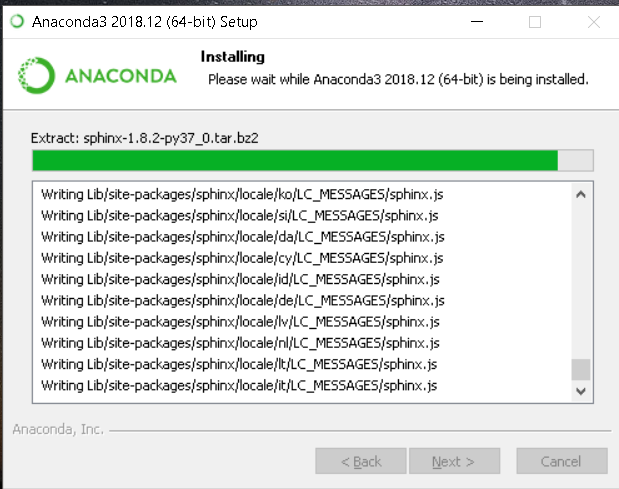
\includegraphics[width=10cm]{figures/fahmi/1.png}
		\centering
	\end{figure}

    \item Instalasi telah selesai
	 \begin{figure}[H]
		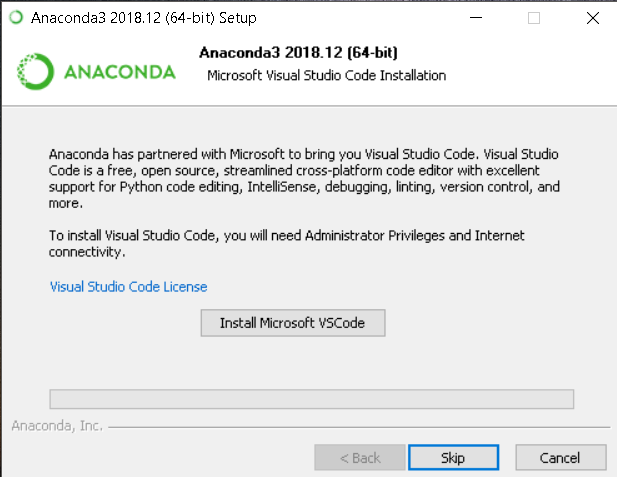
\includegraphics[width=10cm]{figures/fahmi/2.png}
		\centering
	\end{figure}
	
\end{enumerate}
	

\subsection{Penggunaan Spider}
Spyder merupakan text editor dari anaconda dimana di tools ini bisa menjalankan perintah-perintah dengan klik run saja. 
Di anaconda sendiri mempunyai beberapa text editor untuk python tapi yang akan dijelaskan kali ini menggunakan spyder.

Spider sendiri sudah terinstall bersama pada saat kita menginstall Anacoda tadi.

ini adalah contoh tampilan pada Spider.
\begin{figure}[H]
		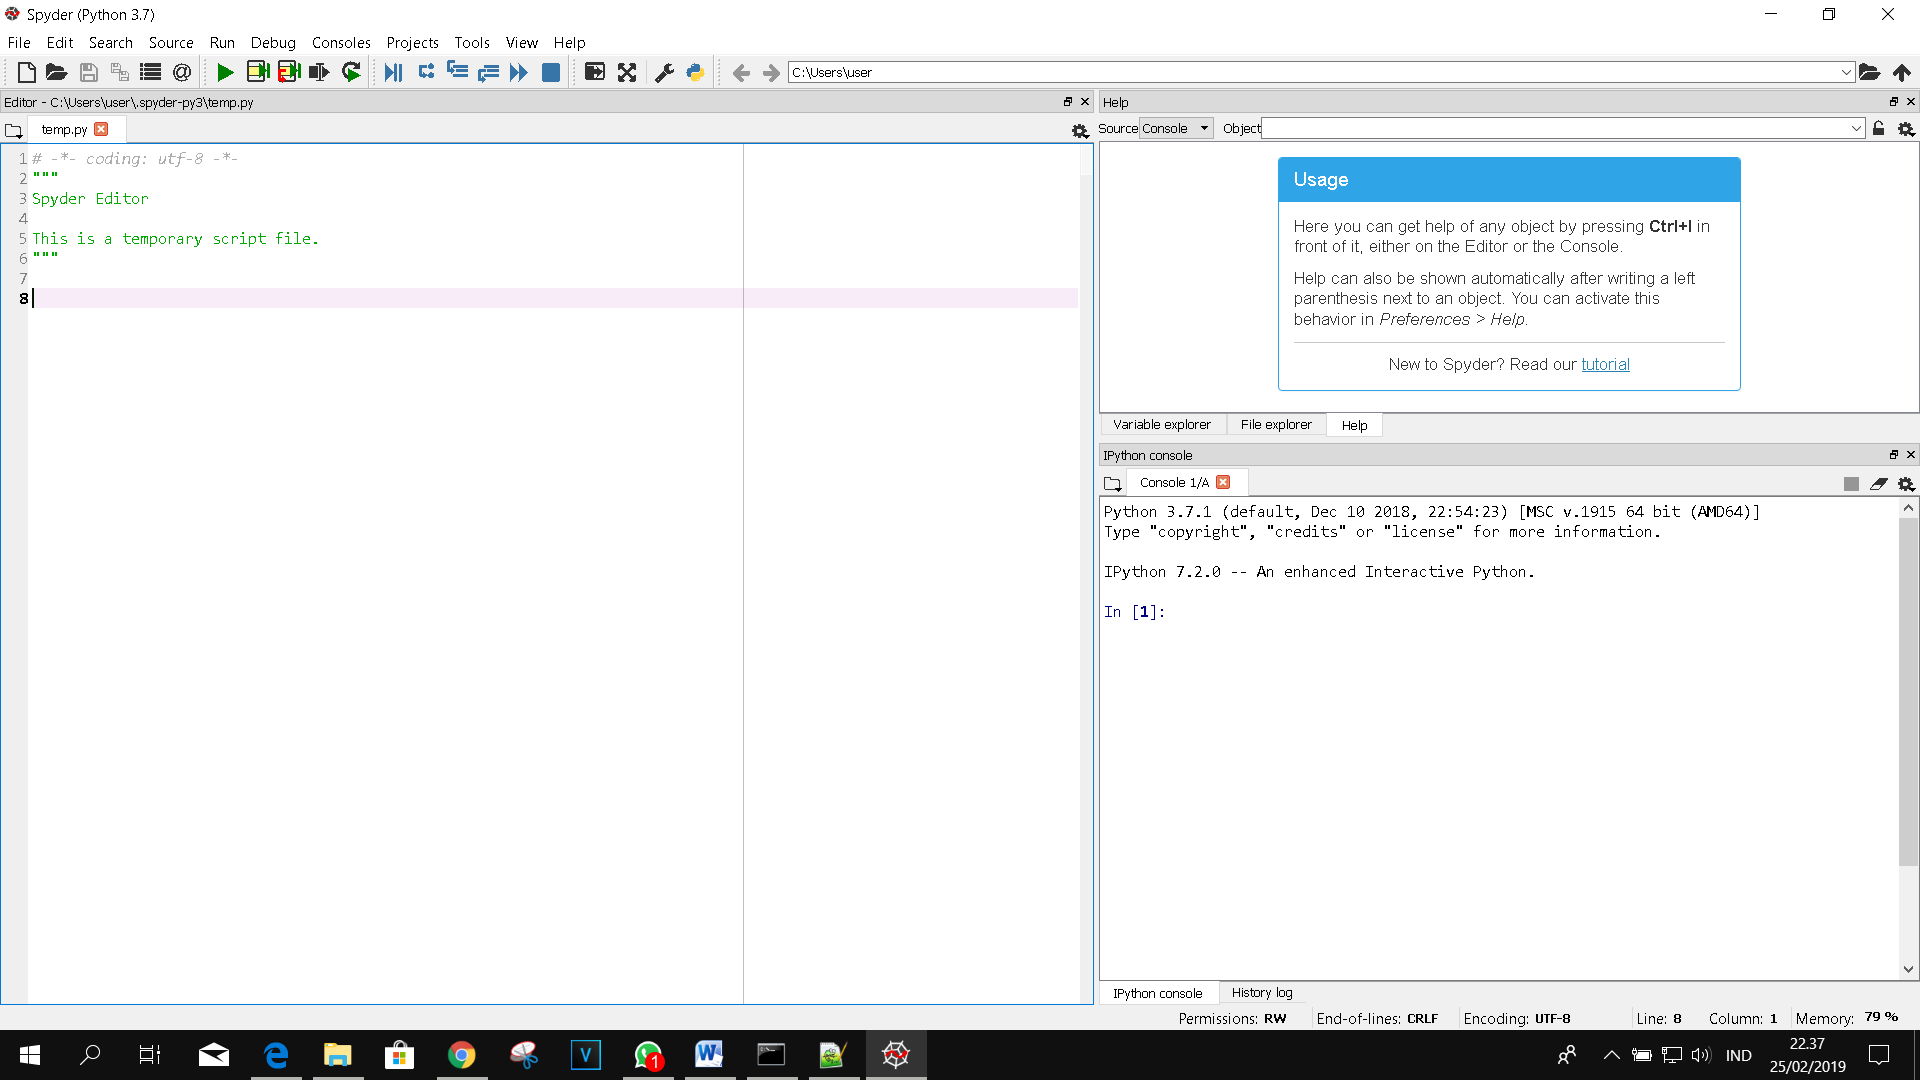
\includegraphics[width=10cm]{figures/fahmi/3.png}
		\centering
	\end{figure}
